% 正文开始
% Chapter 1: Introduction
\section{Introduction}

\subsection{Problem Background}
Sailing, as an ancient sport, is not only one of the water sports in the Olympic Games, but also reflects the consumption level and consumption preference of different regions through the price of sailing. Studying the prices of sailing boats in different regions can pro-vide reference for sailing brokers and offer buying suggestions for sailing enthusiasts, thus promoting the development and progress of local economy.

Sailboats can be divided into two categories: monomer and catamaran, whose types have different impacts on the price. Therefore, separate study of these two types of sailboats is more conducive to the selection and comparison of sailing brokers and sailing enthusiasts.
\begin{figure}[htbp]
    \centering    
    \subfigure[jeanneau60-Monohulled Sailboats(left)]{				% 图片1([]内为子图标题)						
    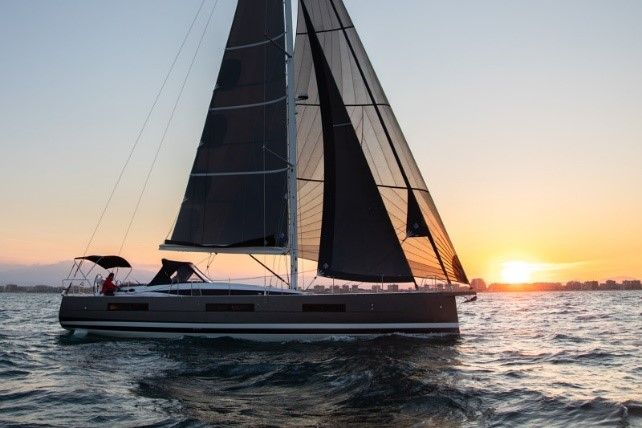
\includegraphics[width=0.45\textwidth]{test_1.jpg}}			  % 子图1的图片宽度 不能空行
    \subfigure[excess15-Catamarans(right)]{				% 图片2
    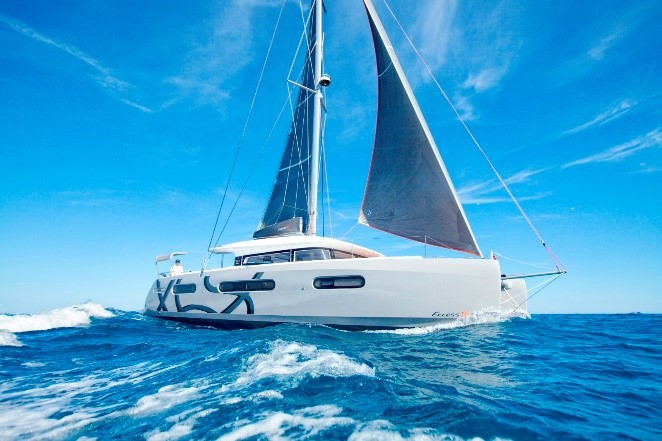
\includegraphics[width=0.45\textwidth]{test_2.jpg}}
	\caption{Comparison of monohull and catamaran} % 图片标题 
\end{figure}
\vspace{-1cm}
\subsection{Restatement of the Problem}
Considering the background information and restricted conditions identified in the problem statement, we need to solve the following problems:

\begin{itemize}
\setlength{\parsep}{0ex} %段落间距
\setlength{\topsep}{2ex} %列表到上下文的垂直距离
\setlength{\itemsep}{1ex} %条目间距
\item Problem 1: We need to build a model to predict the price of different types of sailboats based on some of their characteristics (e.g. beam, drainage, draft, etc.). The accuracy of estimating the price of sailing variety is also discussed.
\item Problem 2: We need to use the above model to discuss the regional consistency of sailing variants and give the actual statistical significance and practical signifi-cance according to the listed price data of sailing vessels in various regions.
\item Problem 3: We need to discuss the role of geographical modelling in the Hong Kong market. By comparing the listing price data, discuss the influence of Hong Kong on the price of monohull and catamaran and whether they are the same.
\item Problem 4\&5: We need to find interesting or meaningful conclusions based on the available data and models, and present our analysis and conclusions to Hong Kong sailing brokers.
\end{itemize}

\subsection{Our Work}
These problems required us to explore the impact of used sailboat parameters and regional effects on sailboat prices. Our work mainly includes:

\begin{itemize}
\setlength{\parsep}{0ex} %段落间距
\setlength{\topsep}{2ex} %列表到上下文的垂直距离
\setlength{\itemsep}{1ex} %条目间距  这三句如果删除就是各条贴在一起
\item First, we use ismissing function and Z-score method to check missing values and outliers.
\item We reduce the dimension of 12 sailboat indexes to 6 indexes, and then use random forest(RF), BP neural network and CNN neural network, and SCA optimization algorithm to optimize the fusion model of the three indexes, and discuss the error of price prediction.
\item For the study of the regional effects of sailing prices, a total of four indicators re-lated to sailing were selected and multiple regression analysis was used. We then calculated the regional effect indicators for the sailing variant to assess the region-al effect of sailing prices.
\end{itemize}

\begin{figure}[htbp]  %h此处,t页顶,b页底,p独立一页,浮动体出现的位置
\centering  %图表居中
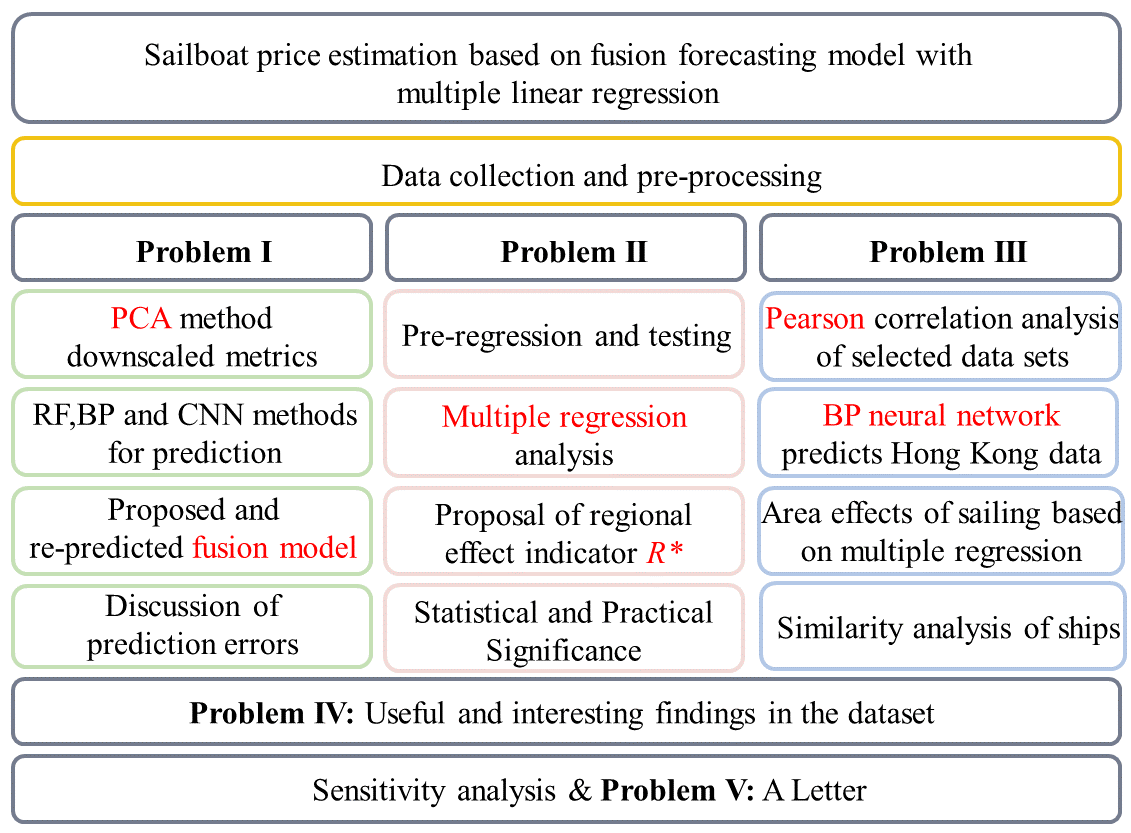
\includegraphics[width=.85\textwidth]{test_3.png} %图片的名称或者路径之中有空格会出问题 
\caption{Flow Chart of this Paper's Research} % 图片标题 
\end{figure}
\vspace{-1cm}
%————————————————————————————————————————————————————————————————————————%

\section{Assumptions and Explanations}
Considering that practical problems always contain many complex factors, first of all, we need to make reasonable assumptions to simplify the model, and each hypothesis is closely followed by its corresponding explanation:
\begin{enumerate}[\bfseries \textit{Assumption} 1:]
	\item \textbf{We assume that there is no major financial crisis or credit crisis in the years under study.}\\
	\textbf{\textit{Explanation:}}The financial crisis will cause the global commodity prices to fluctuate greatly, which is not in line with the general law of commodity development and is not conducive to the establishment of the model.
	\item \textbf{We assume that commodities such as sailboats are traded globally on a normal ba-sis without economic sanctions between countries.}\\
	\textbf{\textit{Explanation:}}When economic sanctions occur between countries, competing countries will ma-liciously inflate or downgrade their own goods to hit the rest. This is not in line with the development of commodity prices, and politically induced price changes should also be excluded.
	\item \textbf{We assume the same level of wear and tear on the sailboat.}\\
	\textbf{\textit{Explanation:}}Since the price of a sailboat is influenced by the degree of wear and tear, etc. on the sailboat itself. This is partly a loss due to changes in the sailboat itself and is not considered during the study.
	\end{enumerate}
Additional assumptions are made to simplify analysis for individual sections. These assumptions will be discussed at the appropriate locations.

%————————————————————————————————————————————————————————————————————————%
\section{Notations}
Some important mathematical notations used in this paper are listed in Table 1. 
\begin{table}[htbp]
\begin{center}
\caption{Notations used in this paper}
\begin{tabular}{c c c}
\toprule[2pt]
\multicolumn{1}{m{1.5cm}}{\centering Symbol}
&\multicolumn{1}{m{12.5cm}}{\centering Description }
&\multicolumn{1}{m{1cm}}{\centering Units}\\
\midrule
$\lambda_i$& Principal Components after Dimensionality Reduction&/ \\
$y_i$& Forecasts of Sailboat Prices&/\\
$a_i$& Weights of each Method in Model Fusion&/\\
$\Delta R$&Changes in Sailing Rankings&/ \\
$R^*$ & Indicators of Regional Effects on the Selling Price of Sailboats &/\\
\bottomrule[2pt]
\end{tabular}\label{tb:notation}

 \begin{tablenotes}
        \footnotesize
        \item[*] *There are some variables that are not listed here and will be discussed in detail in each section. %此处加入注释*信息
      \end{tablenotes}
\end{center}
\end{table}
\vspace{-1.2cm}%在\end{table}下加一行\vspace{-1cm} 其中-1的作用是缩短与下方文字距离的 切记!必须是负数

%————————————————————————————————————————————————————————————————————————%
\section{Model Preparation}
\subsection{Data Overview}
For a large amount of data, it is necessary to process and clean the data before building the model. So we first use the ismissing function to find the missing value and get the miss-ing value as follows:
\begin{table}[H]%浮动体的htbp可以强制在原位显示,改参数为H
  \begin{center}
  \fontsize{12pt}{13.8}\selectfont
  \caption{Missing Data in Given Data}
  \resizebox{\textwidth}{!}
  {\begin{tabular}{c c c c c c c c}
  \toprule[2pt]
  \multicolumn{1}{m{3cm}}{\centering \textbf{Type}}
  &\multicolumn{1}{m{2cm}}{\centering \textbf{Make}}
  &\multicolumn{1}{m{2cm}}{\centering \textbf{Variant}}
  &\multicolumn{1}{m{2cm}}{\centering \textbf{Length}}
  &\multicolumn{1}{m{2cm}}{\centering \textbf{Geographic}}
  &\multicolumn{1}{m{2cm}}{\centering \textbf{State}}
  &\multicolumn{1}{m{2cm}}{\centering \textbf{Price}}
  &\multicolumn{1}{m{2cm}}{\centering \textbf{Year}}
  \\ %m后面是列宽
  \midrule
  \multirow{3}*{\makecell[c]{Mono-hulled\\Sailboats}}&Beneteau&Oceanis 54&54&USA&-&\$479,805&2013 \\
  ~ &Delphia&46 cc&46&Europe&-&\$314,606&2013  \\
  ~ &Bavaria&Cruiser 46&46&Europe&-&\$201,640&2014\\ 
  Google Scholar&\multicolumn{7}{c}{This type has NO missing value} \\
  \bottomrule[2pt]
  \end{tabular}}
  \end{center}
\end{table}
\vspace{-1cm}
We remove the above missing values and then use the Z-score method to handle the outliers. Finally, we found that there were no outliers in the original data set.In addition, other data collected in this paper have been processed by the above method.
\subsubsection{Data Collection}
The official website of FEC in Victoria, Australia was queried and lots of data about wildfires were obtained. And other data sources are shown in Table 2.
\upcite{1}\upcite{2}\upcite{3}\upcite{4}\upcite{5}
\begin{table}[H]
  \begin{center}
  \caption{Data and Database Websites}
  \resizebox{\textwidth}{!}
  {\begin{tabular}{c c}
  \toprule[2pt]
  \multicolumn{1}{m{6.5cm}}{\centering \textbf{Database Names}}
  &\multicolumn{1}{m{10cm}}{\centering \textbf{Database Websites} }\\ %m后面是列宽
  \midrule
  GDP of Each Country& https://ourworldindata.org/ \\
  GDP of Some European Countries & https://data.worldbank.org/ \\
  \multirow{2}*{Partial Sailing Parameters}& https://www.sailboat-cruising.com/\\ 
  ~& https://sailboatdata.com/ \\
  \bottomrule[2pt]
  \end{tabular}}
  \end{center}
  \end{table}
  
  \vspace{-1cm}
\subsubsection{Data Screening}
According to the data given, we find that the price of sailboats is not only related to the brand and the time of delivery, but also to the selling area. This is because the actual price of sailing ships is often affected by local economic conditions, so we collected European and American GDP data and visualized it.
\upcite{1}\upcite{2}\upcite{3}\upcite{4}\upcite{5}
\begin{figure}[htbp]
    \centering    
    \subfigure[European GDP Per Capita(left)]{				% 图片1([]内为子图标题)						
    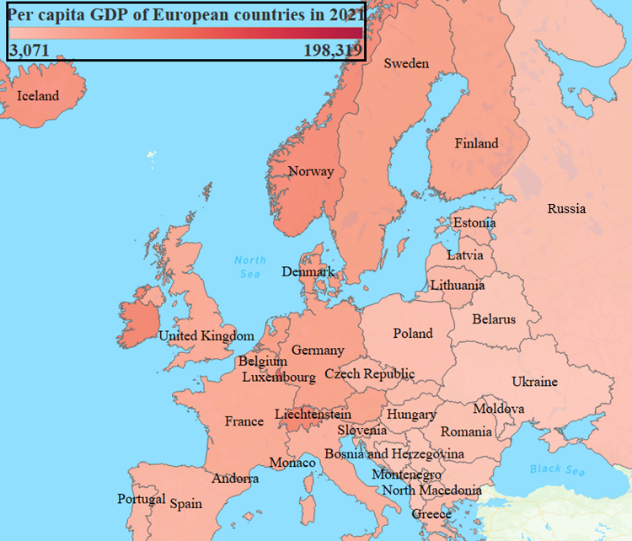
\includegraphics[width=0.45\textwidth]{test_4.png}}			  % 子图1的图片宽度 不能空行
    \subfigure[Part of U.S.GDP per Capita(right)]{				% 图片2
    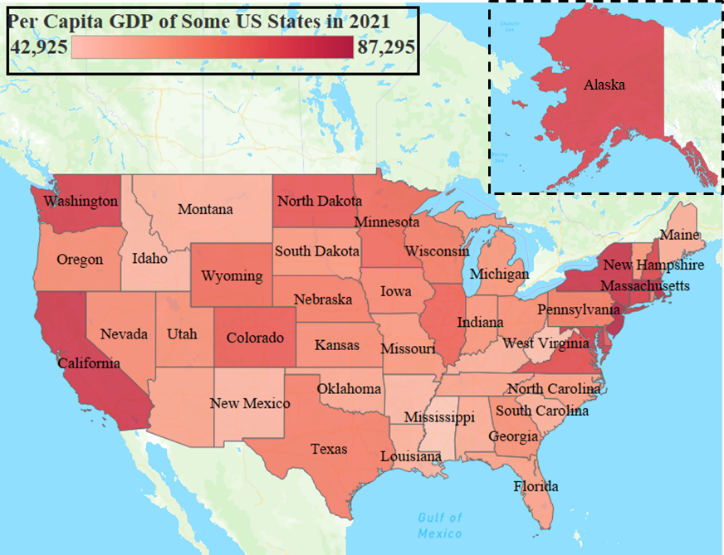
\includegraphics[width=0.505\textwidth]{test_5.png}} 
	\caption{Data Screening} % 图片标题 
\end{figure}


It is reasonable to predict the price of sailing boats according to the above indexes, which will affect the performance, sailing ability, comfort and service life of sailing boats. Therefore, they are all factors that sailing enthusiasts and sailing brokers need to consider when evaluating the price of sailing boats. At the same time, the importance and weight of these indicators may vary with the type, age, brand and other factors. Therefore, factors such as selling location, brand of sailing boat and year of manufacture were also considered when building the model below.
\begin{table}[H] %浮动体的htbp可以强制在原位显示,改参数为H
  \begin{center}
  \caption{Partial Monohull and Catamaran data}
  \resizebox{\textwidth}{!}
  {\begin{tabular}{c c c c c c}
  \toprule[2pt]
  \multicolumn{1}{m{4cm}}{\centering \textbf{/}}
  &\multicolumn{1}{m{2cm}}{\centering \textbf{Beam length$/m$}}
  &\multicolumn{1}{m{2cm}}{\centering \textbf{Draft/m$^3$}}
  &\multicolumn{1}{m{2cm}}{\centering \textbf{Displacement\\/m$^3$}}
  &\multicolumn{1}{m{2cm}}{\centering \textbf{Sail area/m$^2$}}
  &\multicolumn{1}{m{4cm}}{\centering \textbf{Hull materials}}
  \\ %m后面是列宽
  \midrule
  Bail-4.6&7.2&1.15&11800&116&Carbon fiber \\
  Alliage-AZZURO-53&6.7&1.95&18000&163&Aluminium alloy\\
  \bottomrule[2pt]
  \toprule[2pt]
  \multicolumn{1}{m{4cm}}{\centering \textbf{/}}
  &\multicolumn{1}{m{2cm}}{\centering \textbf{Engine hours/h}}
  &\multicolumn{1}{m{2cm}}{\centering \textbf{Sleeping capacity/person}}
  &\multicolumn{1}{m{2cm}}{\centering \textbf{Headroom\\/m}}
  &\multicolumn{1}{m{2cm}}{\centering \textbf{GDP/\\Trillion\$}}
  &\multicolumn{1}{m{4cm}}{\centering \textbf{-}}
  \\ %m后面是列宽
  \midrule
  Bail-4.6         &2000 &12  &21.87&4.08&- \\
  Alliage-AZZURO-53&4000 &6~8 &17.00&2.56&-\\
  \bottomrule[2pt]
  \end{tabular}}
  \end{center}
\end{table}
\vspace{-1cm}
It is reasonable to predict the price of sailing boats according to the above indexes, which will affect the performance, sailing ability, comfort and service life of sailing boats. Therefore, they are all factors that sailing enthusiasts and sailing brokers need to consider when evaluating the price of sailing boats. At the same time, the importance and weight of these indicators may vary with the type, age, brand and other factors. Therefore, factors such as selling location, brand of sailing boat and year of manufacture were also considered when building the model below.


